\section{Implementierung} \label{sec_04}

\subsection{Projektarchitektur}
Wie in Abschnitt 3 gezeigt, besitzt das Projekt verschiedene Teile, welche miteinander kommunizieren. Die Architektur aus dem Grobkonzept wird größtenteils übernommen. Lediglich die Kommunikation mit dem Sprachassisstenten wird von dem Main Controller übernommen.

\begin{figure}[H]
\centering
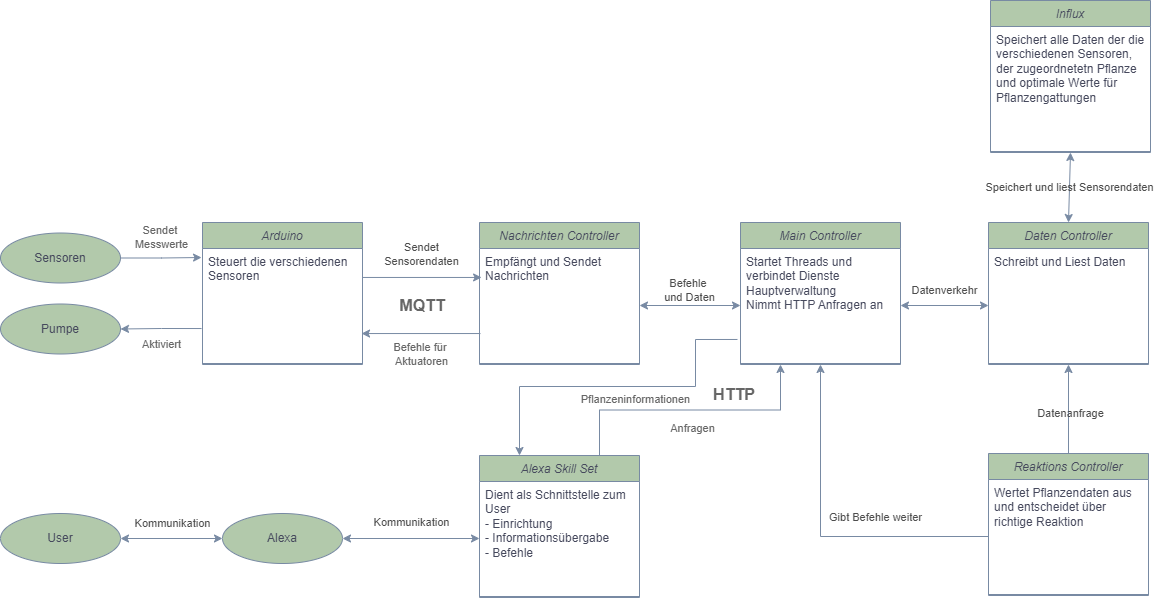
\includegraphics[width=\textwidth]{images/Feinkonzept_Flow.drawio.png}
\caption{Flowchart der Software-Architektur}\cite{rainpoint_smart_timer}
\label{fig:grob_flow}
\end{figure}

An den Arduino-Mikrocontroller sind verschiedene Sensoren angeschlossen. Dieser sendet hierbei Daten, und erhält Anweisungen, über einen MQTT-Kanal mit dem Main Controller, welche Aufgaben an andere Controller verteilt. Diese laufen auf einem Universitätserver. Hier werden Daten aufgenommen, gesendet, geschrieben, gelesen und ausgewertet.

\subsection{I/O der Hardware}
Der Arduino-Microcontroller besitzt zahlreiche Anschlüsse um verschiedenste IoT-Projekte zu unterstützen. Über ein Steckbrett wurden die verschiedenen Leitungen mit dem Microcontroller verbunden.

Die verschiedenen Sensoren benötigten hierfür jeweils Stromein- und ausgang. Boddenfeuchtigkeit und Lichtwerte wurden über analoge Eingänge aufgenommen. Der Temperatur- und Luftfeuchtigkeitssensor wurde über einen digitalen Eingang mithilfe einer I2C-Schnittstelle an den Microcontroller angebunden. Die Pumpe erhält das Signal zum Ein- und Ausschalten über einen digitalen Ausgang.

\subsection{Mikrocontroller}
Der Mikrocontroller muss folgende Aufgaben bewältigen können:
\begin{itemize}
    \item Initialisierung der Sensoren
    \item Messung der Werte
    \item Umwandlung der Werte
    \item Senden von Daten
    \item Empfangen von Daten
    \item Einschalten der Pumpe
\end{itemize}

Diese Aufgaben werden in einer C++-Datei, mit einer zugehörigen yaml-Datei für verschiedene Parameter bewältigt.

Die verschiedenen Sensoren wurden an den Mikrocontroller angeschlossen und können so ausgelesen werden.

\begin{figure}[H]
\centering
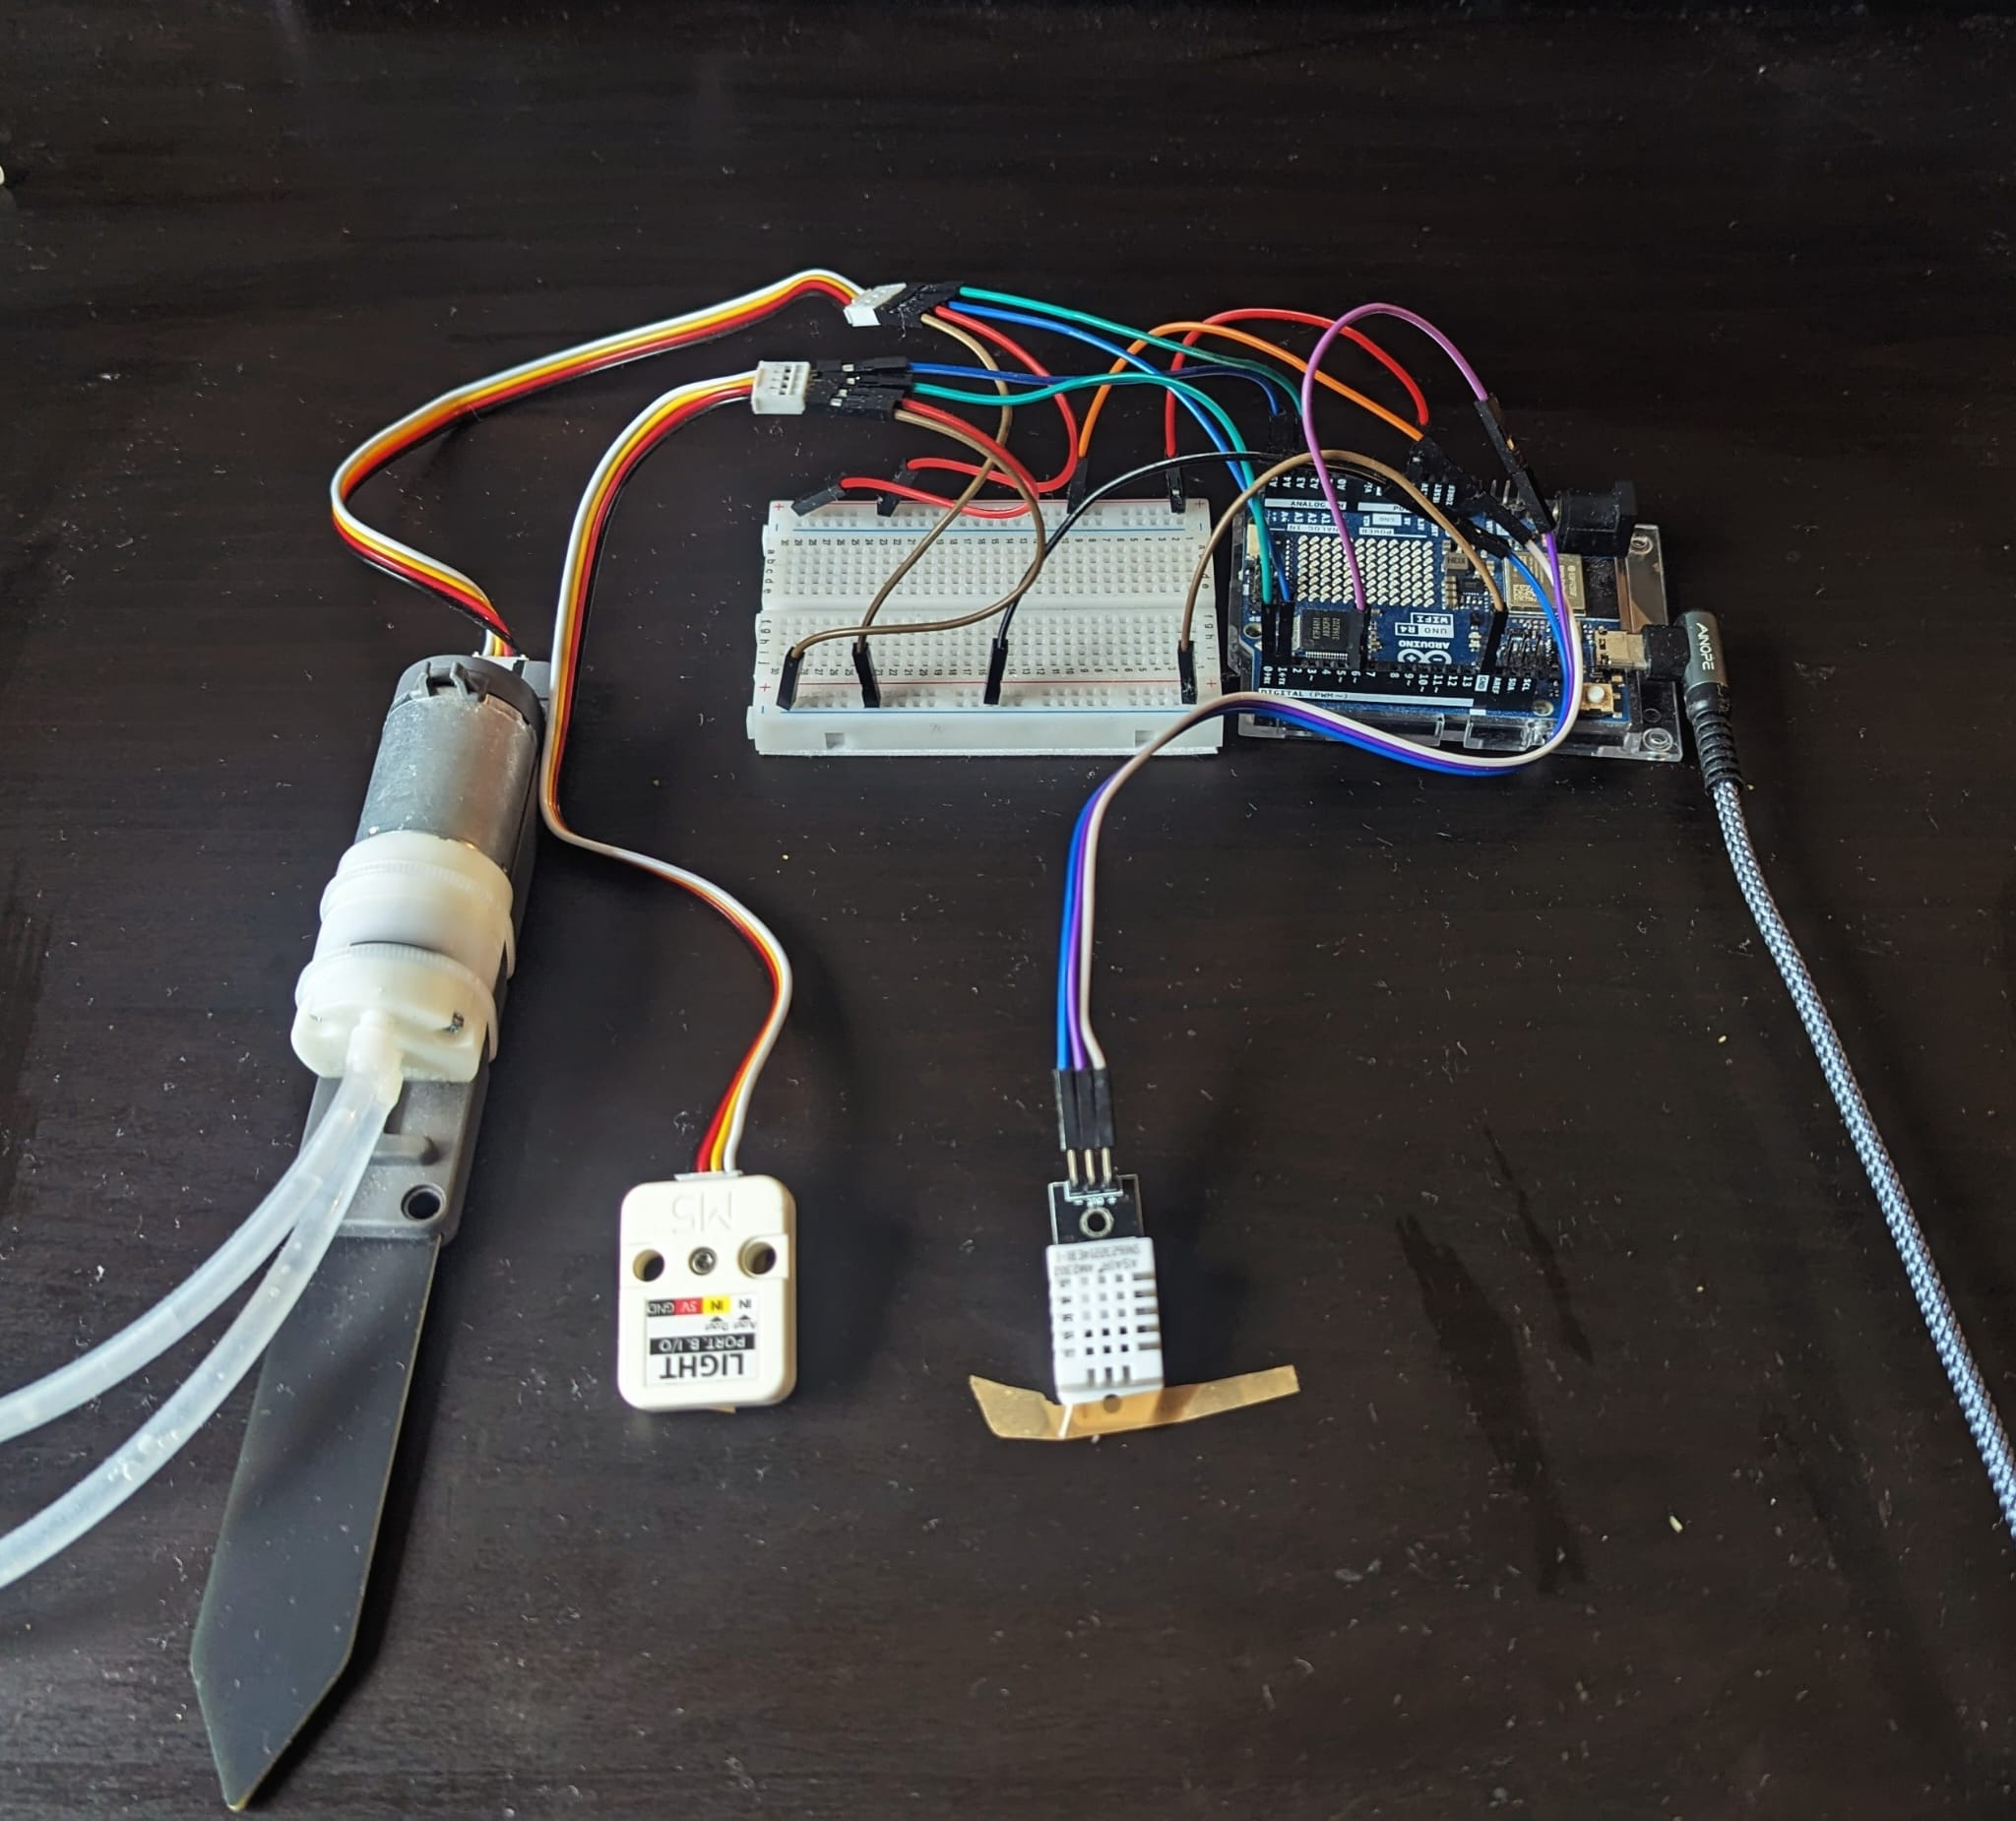
\includegraphics[width=\textwidth]{images/microcontroller.jpg}
\caption{Mikrocontroller mit Sensoren, (v.l.n.r.) Pumpe & Bodenfeuchtigkeit, Temperatur & Luftfeuchtigkeit, Licht}\cite{rainpoint_smart_timer}
\label{fig:rainpointDiagram}
\end{figure}

\subsubsection{Sensormessung und Umwandlung der Daten}
Nach der Zuweisung der Anschlüsse des Boards, konnten die meisten Sensoren mittels eines analogen Inputs ausgelesen werden. Diese konnten so ohne weitere Installation oder spezifische Bibliotheken ausgelesen werden. Lediglich der Sensor für Temperatur und Luftfeuchtigkeit benötigt die spezifische Bibliothek "DHT". Dessen Werte wurden über den I2C Bus ausgelesen.

Die genaue Messung der Bodenfeuchtigkeit variiert geringfügig je nach Sesnor, sie mussten daher zunächst kalibriert werden. Nach einigen Tests wurde herausgefunden dass für diesen speziellen Sensor 370 eine maximale  und 795 eine minimale Bodenfeuchte bedeutet. So kann die Feuchtigkeit mittels einfacher Rechnung in Prozent ausgedrückt werden.

\subsubsection{Senden und Empfangen von Daten}
Die interne WLAN-Bibliothek "WiFiS3" wurde benutzt, um den Arduino mit dem Internet zu verbinden. Diese ist jedoch nicht völlig stabil, bei Netzwerkproblemen kann die Verbindung getrennt werden und wird nicht automatisch wieder aufgebaut. Um das Problem zu lösen wird vor dem Senden einer Nachricht der Status der WLAN-Verbindung nachgefragt. Besteht diese nicht, wird die Verbindung erneut hergestellt.

Mithilfe der Bibliothek "ArduinoMqttClient" kann zuverlässig eine MQTT Verbindung hergestellt werden. Hierbei wird auch ein Empfänger eingerichtet.

Über das zutreffende Topic wird der reine Datenwert (payload) des Sensors geschickt.

Erhält der Mikrocontroller eine Nachricht auf dem Topic zur Pumpenaktivierung wird diese Funktion gestartet.

\subsubsection{Einschalten der Pumpe}
Der Payload der MQTT-Nachricht zur Pumpenaktivierung erhält in bit-Form die zeitliche Dauer, wie lange die Pumpe pumpen soll. Nach dem Umwandeln in einen Integer, wird die Pumpe für so viele Sekunden aktiviert. Um Fehler und Manipulation vorzubeugen kann die Pumpe maximal zehn Sekunden lang am Stück pumpen.

\subsubsection{Zusammenfassung}

Der vollständige Versuchsaufbau sieht wie folgt aus:

\begin{figure}[H]
\centering
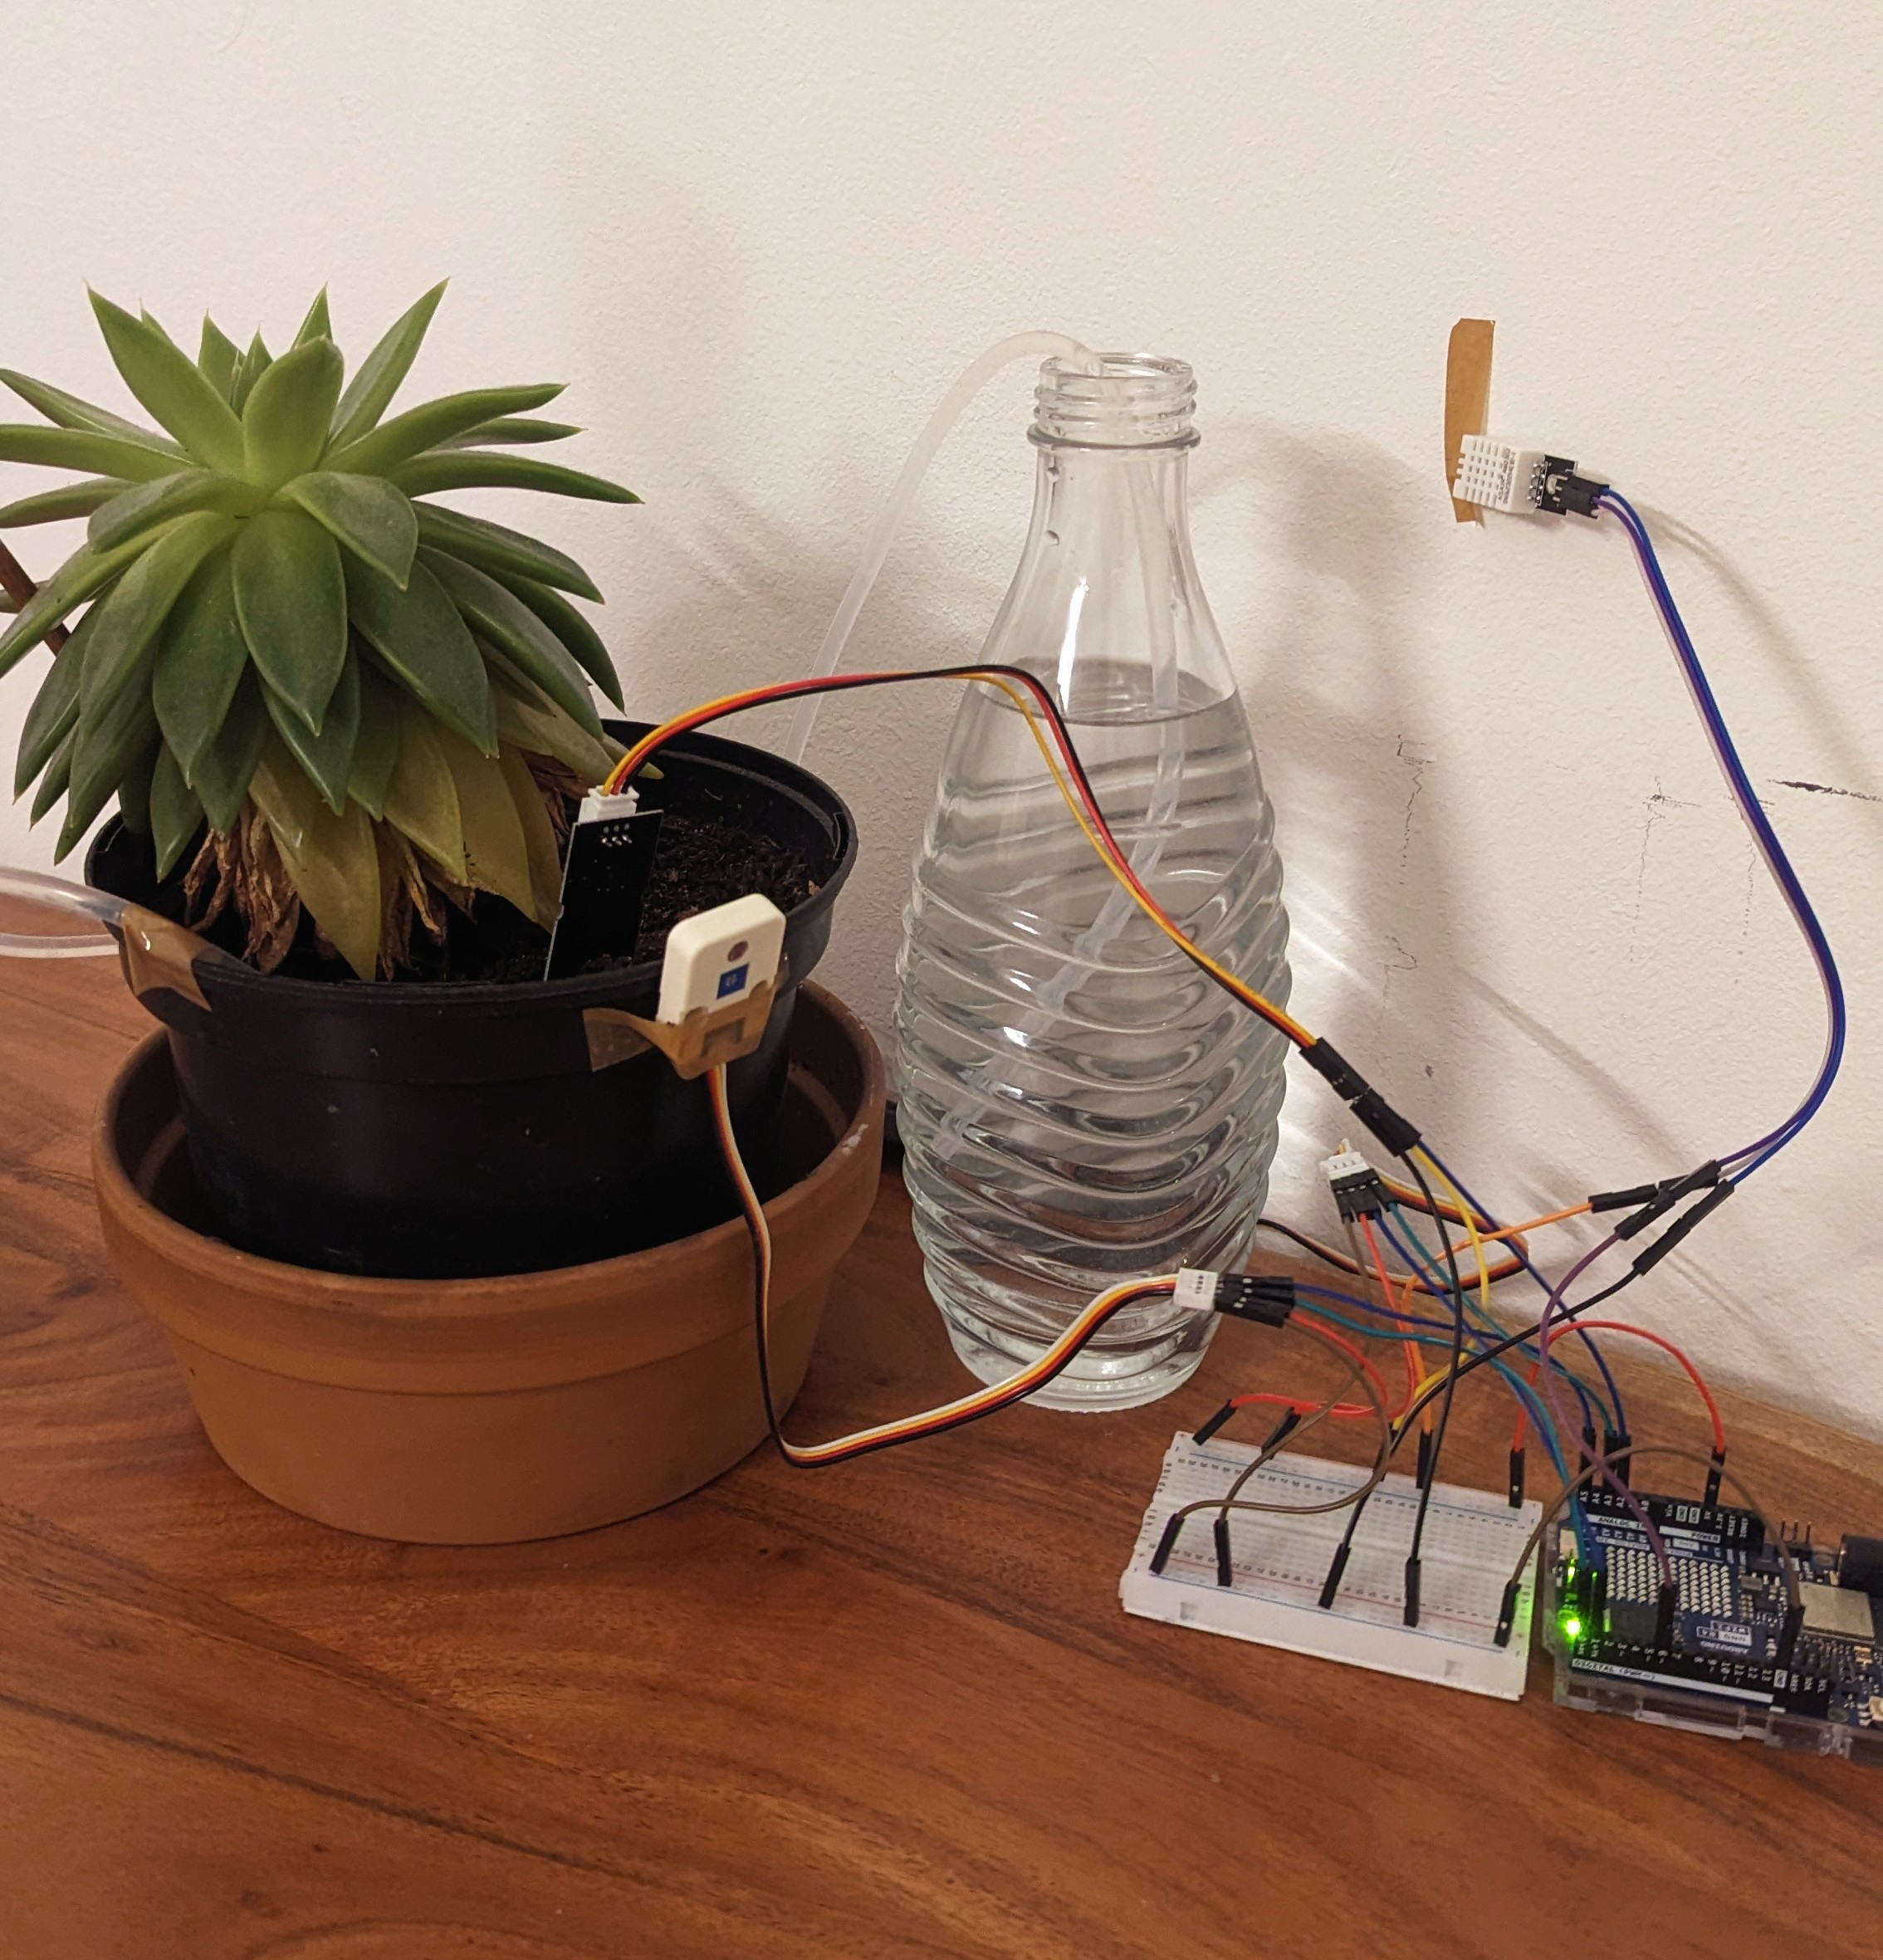
\includegraphics[width=\textwidth]{images/versuchsaufbau.jpg}
\caption{Aufgebautes Gerät}\cite{rainpoint_smart_timer}
\label{fig:rainpointDiagram}
\end{figure}

\subsection{Main Controller}
Der Main Controller dient als Steuerungseinheit. Er verwaltet die verschiedenen Tätigkeiten und verbindet die Dienste miteinander.

Der Standard Python-Logger wurde benutzt, um die Entwicklung, insbesondere in der Docker-Umgebung, zu vereinfachen und leichter nachzuvollziehen.

Parameter werden generell immer in externen yaml-Dateien gespeichert, und mit einer gesonderten Datei importiert. Hier wird überprüft, ob alle nötigen Parameter gespeichert sind und nur diese werden dann ausgewählt.

Der Main-Controller arbeitet hierbei in drei verschiedenen Threads. Einer für den Empfang von MQTT-Daten, einer für die regelmäßige Abfrage der gespeicherten Datenbank-Daten und einer zum Erhalten von HTTP-Anfragen des Sprachcontrollers. Diese werden über den Standard Python-Threader initialisiert.

Momentan werden alle Daten als Werte für eine Sukkulente gespeichert. Später soll die Datenbank selbst zuordnen welches Gerät, welche Pflanze enthält.

\subsection{Nachrichten Controller}
Der Nachrichten Controller verwaltet die Kommunikation über MQTT mit dem Mikrocontroller.

Mithilfe des MQTT-Clients kann eine stabile Verbindung zu einem MQTT-Kanal hergestellt werden, über den alle nötigen Nachrichten empfangen und gesendet werden können. Der Mikrocontroller schickt hierbei vier Nachrichten für Licht, Temperatur und Luft- und Bodenfeuchtigkeit. Diese werden getrennt voneinander verarbeitet.

\subsection{Datenbankcontroller}

\subsubsection{Schreiben der Daten}
Zunächst wird im die Influx-Instanz mit den richtigen Parametern initiiert. 
Erhält der Controller eine Nachricht wird das Topic (z.B. Temperatur) richtig zugeordnet. Stimmt das Topic nicht mit der internen Liste überein wird es nicht weiter verarbeitet. So können weitreichende Fehler vermieden werden.

Der Payload der Nachricht wird in einen Float umgewandelt und in die passende Tabelle geschrieben. Später wird für jedes Gerät eine eigene Tag-Nummer erstellt.

Ist dies der erste Eintrag in der Tabelle wird diese automatisch von Influx erstellt.

\subsubsection{Lesen der Daten}
Die No-SQL Anfrage für das Lesen der gespeicherten Daten sieht folgendermaßen aus:

\begin{verbatim}
<f"""from(bucket: "{bucket}")
                |> range(start: -5m)
                |> filter(fn: (r) => r._ measurement == "{table_ name}")
                |> mean()""">
\end{verbatim}

Der Durchschnitt der letzten fünf Minuten wird aus der entsprechenden Tabelle, beispielsweise Temperatur, entnommen. Nach einer Überprüfung, ob ein sinnvolles Ergebnis erzielt wurde, wird der Wert weitergegeben.

\subsection{Reaktionscontroller}
Der Reaktionscontroller benutzt simple Decision Trees, um die richtige Reaktion für derzeitige Umweltkonditionen zu finden. 

Regelmäßig werden die Werte der Klasse PlantSensorData überschrieben. Die Klasse enthält die aktuellen Werte der Pflanze und die derzeitige Uhrzeit.

Die derzeitigen Werte werden aus der Datenbank gelesen und dem richtigen Attribut zugeordnet. Falls die Tabelle leer ist, wird explizit nichts zurückgegeben und eine Warnung ausgegeben. Dies ist unter anderem beim erstmaligen Starten der Fall, wenn noch keine Daten von den Sensoren erhalten wurden.

Die optimalen Werte für verschiedene Pflanzen sind in einer CSV-Tabelle gespeichert. Diese Werte wurden aus Erfahrungsberichten von Experten zusammengestellt und können jederzeit verändert werden. In dieser sind, der Pflanzengattung zugeordnet, die Werte gespeichert, in denen sich die reale Pflanze befinden sollte, um optimal zu wachsen. Bei einer späteren KI-Integrierung sollen diese Werte von dem System selbst und nicht von Experten angepasst werden.

Die Tabelle für die Sukkulenten sieht folgendermaßen aus:

\begin{table}
    \centering
    \begin{tabular}{|p{5cm}|p{7cm}|}
         Plant Name&Succulent \\ \hline
         Temperature min (C)&4 \\ \hline
         Temperature max (C)&27 \\ \hline
         Humidity min (rH)&40 \\ \hline
         Humidity max (rH)&50 \\ \hline
         Moisture min&33 \\ \hline
         Moisture max&45 \\ \hline
         Sun min (h)&6 \\ \hline
         Sun Category&direct \\ \hline
         Notes&Grows the best if it has constant, strong light. Should lay a bit in the shade. Be careful of direct sun. Ideally they should get a lot of air circulation. \\ \hline
    \end{tabular}
    \caption{Tabelle für Sukkulenten}
    \label{tab:my_label}
\end{table}

"Moisture min" und "Moisture max" sind in Prozent angegeben. "Notes" sind insbesondere für die Nutzenden gedacht, um bei der Pflanzenpflege zu helfen.

Um die Daten zu vergleichen sucht ein Algorithmus nach dem richtigen Eintrag in der Tabelle, und speichert diese in einer Klasse namens OptimalPlant.

Besonderer Fokus lag auf dem automatischen Bewässern der Pflanze. Der echte Wert der Bodenfeuchtigkeit wird mit den optimalen Werten verglichen. Liegt dieser darunter wird eine Funktion zur Aktivierung der Pumpe gestartet. Ein adäquates Ergebnis oder ein zu hoher Wert wird dem Nutzer mitgeteilt. Ähnlich gestalten sich die anderen Abfragen.

\subsection{Sprachsteuerungs Controller}
Die Implementierung eines Sprachsteuerungscontrollers mit Alexa Skills, erfordert einen neuen Skill in der Alexa Developer Console. Hier wird ein neues Interaktionsmodell kreirt. Intents sind hierbei die generellen Befehle, während Slots verschiedene Variablen repräsentieren.

Ein Interaktionsmodell sieht so wie folgt aus:

\begin{verbatim}
    {
  "intents": [
    {
      "name": "PlantInfoIntent",
      "slots": [],
      "samples": [
        "give me information about my plant",
        "tell me about my plant",
        "what does my plant need",
        "how is my plant"
      ]
    },
    {
      "name": "AMAZON.HelpIntent",
      "samples": []
    },
    {
      "name": "AMAZON.CancelIntent",
      "samples": []
    },
    {
      "name": "AMAZON.StopIntent",
      "samples": []
    }
  ]
}
\end{verbatim}

In diesem können verschiedene Sprachbefehle für einen Skill gelistet werden. Mit den Samples von PlantInfoIntent kann die normale Funktion des Sfkills aktiviert werden. die anderen Intents sind von Amazon vorgegeben, sie enthalten Phrasen wie "help", "how do I use this skill", "nevermind" oder "stop". Bei bedarf können hier weitere Phrasen hinzugefügt werden.

Hiernach muss in der AWS Lambda Konsole der zugehörige Python-Code geschrieben werden, welcher das Backend durch eine HTTP Anfrage aufruft. Sagt der Nutzende nach dem Aktivieren des Skills eine der Phrasen auf, wird der zugehörige Python-Code aktiviert.

\subsection{Testing}
Zur Übersicht des Projektes wurde ein "Feature" zum Management der Bodenfeuchtigkeit erstellt. Dieses wurde in Cucumber geschrieben, um als Kommunikation zwischen Projektleiter und Entwickler zu stehen. 

Das Feature sieht folgendermaßen aus:
\begin{verbatim}
Feature: Moistere Level Management
    Scenario Outline: Moisture level <scenario_name>
        Given an intelligent vase which is ready to manage soil moisture
        And the vase holds a <plant_type>
        And we have a list of optimal environment for plants where we can search
        the matching plant <plant_type>
        And that plant requires an optimal moisture level between
        <min_optimal> and <max_optimal>
        When the plant has an average moisture level of <average_moisture>
        Then <expected_action> should happen

        Examples:
            |scenario_name |min_optimal|max_optimal|average_moisture|expected_action
            |Below optimal |8          |12         |5               |Activate Pump 
            |Optimal       |8          |12         |10              |Do Nothing  
            |Too high      |8          |12         |15              |Alert User    
\end{verbatim}

Nach der Implementation der richtigen "Steps" konnte dieser Test am Ende ohne Fehler durchlaufen werden.

Zusätzlich wurden mehrere Unit-Tests erstellt, um die Funktionsweise von Code-Einheiten zu testen, und sicherzustellen, dass verschiedenste Fälle abgedeckt sind. Hierzu gehören unter anderem die Reaktion auf verschiedene Arten von MQTT-Nachrichten, wie etwa das falsche Topic oder ein falscher Payload oder das Überprüfen einzelner Funktionen wie das Suchen einer bestimmten Pflanze in der CSV-Datei.

\subsection{Deployment}
Für das Deployment wurden GitHub und Docker benutzt.

GitHub diente als Versionskontrolle und als Testingtool. Bei einem push auf den main-branch wurden Workflows aktiviert, um Behave- und Unittests automatisch durchzuführen. Hierbei mussten verschiedene Konfigurationswerte in die Umweltvariablen von GitHub gespeichert werden.

Über DockerHubs werden neue Versionen des Projektes gepublished und auf den Universitätsserver gespielt.

Die Docker-cCmpose Datei installiert hierbei zwei verschiedene Services auf unterschiedlichen Ports, die Influx Datenbank und den Controller-Code. Die Lauffähigkeit von beiden wird mit einen Healthcheck garantiert. Die nötigen Konfigurationselemente erhält sie aus Sicherheitsgründen aus den Umgebungsvariablen des Systems. Zur Vereinfachung der Entwicklung werden hierbei alle bereits vorhandenen Einträge gelöscht, bei Bedarf können diese aber auch langfristig gespeichert werden.